\documentclass{article}
\usepackage{v-problem}
\vgeometry
\usepackage{v-electrostatics}
%\usetikzlibrary{decorations.markings}

\begin{document}
\vtitle[ELECTROSTATICS]

\def\pn{09}
\def\book{Irodov}
\def\page{106}
\def\gdrive{https://drive.google.com/drive/folders/1uNi-9WQ02jZIJU_ppkYAjxs8VdXmQyGs?usp=share_link}

\def\question{
A thin half-ring of radius $R = 20 \cm$ is uniformly charged with a total charge $q=0.70 \, \text{n}\!\Coulomb$. Find the magnitude of the electric field strength at the curvature centre of this half-ring.
}

\vspace*{\fill}
\begin{tikzpicture}
	\node[qnumber] (n) at (0, 0)[scale=2] {$\pn.$};
	\node[question] (q) [right=2mm of n.east] {\question};
	\tzline[divider]<-0.125, 0> (q.north west)(q.south west);
	\node[format] (f) at  (q.south east){[\book \quad \page]};
\end{tikzpicture}	
\vspace*{\fill}

\begin{center}
\begin{tikzpicture}
\tzcoor*(0, 0)(O){$O$}[b]
\foreach \a in {90, 100,..., 270}{
	\tznode(\a:2){$+$}[scale=0.8]
	\tzdot(\a:2)(7pt)
	\tzline[->](\a:1.86)(\a:1.25)
}
\tzline+[->](O)(1.5, 0){$\vec{E}$}[r]
\end{tikzpicture}
\end{center}
\pagebreak

\vtitle[\texttt{Solution}]
\begin{center}
\begin{tikzpicture}
[arcnode/.style 2 args={                
	decoration={
	raise=#1,             
	markings,   
	mark=at position 0.5 with { 
		\node[inner sep=0] {#2};
	}
},
postaction={decorate}},
thick
]
\def\A{6} %angle for element
\def\AA{130} %at angle
\def\r{2} %radius
\def\dr{0.12} %delta r
\def\RO{\r+\dr} %radius outer
\def\RI{\r-\dr} %radius inner
\def\R{1.25}
\tzcoor(\AA:\RO)(O') %point at right end
\tzcoor*(0, 0)(O){$O$}[bl]
	\foreach \a in {90, 100, ..., 270}{
		\tznode(\a:\r){$+$}[scale=0.65]
		\draw(\a:\r) circle [radius=\dr];
	}
	\tzline[dashed, thin]($(O)+(-3, 0)$)($(O)+(3, 0)$)
	\tzlines(O)(\AA+\A:\RO)(O)(\AA-\A:\RO);
	\tzarc(O)(\AA-\A:\AA+\A:\RO)
	\tzarc(O)(\AA-\A:\AA+\A:\RI)
	\tzline[->](O)($(O')!1.5!(O)$){$\d{\vec{E}}$}[r]
	\tzanglemark(\AA-\A:\r)(O)(\AA+\A:\r){$\d{\theta}$}(15pt)
	\tzanglemark(\AA+\A:\r)(O)(180:\r){$\theta$}(15pt)
	\tzanglemark'($(O')!1.75!(O)$)(O)(0:\r){$\theta$}(15pt)
	\tzline+[->](O)(\R, 0){$\d{E}\cos\theta$}[r]
	\tzline+[->](O)(0, -\R){$\d{E}\sin\theta$}[b]
	\tzarc[|<->|, arcnode={-10pt}{$\d{l}$}](O)(\AA-\A:\AA+\A:1.1*\RO)
\end{tikzpicture}
\end{center}

\addtolength{\jot}{2ex}

\begin{align*}
\intertext{Differential electric field($\d{E}$) due to the small arc($\d{l}=r\d{\theta}$) which substends a differential angle($\d{\theta}$) at the center is}
\d{E} &= \K \cdot \dfrac{\d{q}}{r^2}\\
	&= \K \cdot \dfrac{\lambda \cdot r \cdot\d{\theta}}{r^2}\\
	&= \K \cdot \dfrac{q \cdot\d{\theta}}{\pi r^2} ,\quad\quad q=\pi r\lambda
\end{align*}
\pagebreak

\def\I{\int_{-\pi/2}^{\pi/2}}
\begin{align*}
\intertext{Total electric field along x-axis}
E_x &= \I \d{E}_x\\
	&= \I \d{E}\cos\theta\\
	&= \I \K \cdot \dfrac{q \cdot\d{\theta}}{\pi r^2} \cos\theta\\
	&= \K \cdot \dfrac{q}{\pi r^2} \I \cos\theta \d{\theta}\\
	&= \K \cdot \dfrac{q}{\pi r^2} \left[\sin\theta \right]_{-\pi/2}^{\pi/2}\\
	&= \K \cdot \dfrac{2q}{\pi r^2}\\
\Aboxed{E_x &= \dfrac{q}{2\pi^2\varepsilon_0 r^2}=100\V/\m}\ans\\
\intertext{Total electric field along y-axis}
E_y &= \I \d{E}_y\\
	&= \K \cdot \dfrac{q}{\pi r^2} \I \sin\theta \d{\theta}\\
\Aboxed{E_y &= 0}\ans
\end{align*}

\pagebreak

\vspace*{\fill}
\begin{center}
	\fbox{\qrcode[height=2cm]{\gdrive}}
\end{center}
\vspace*{\fill}

\end{document}
